%************************************************
\chapter{Value Iteration with CVaR}\label{ch:vi}
%************************************************

Value iteration is a standard algorithm for maximizing expected discounted reward used in reinforcement learning. In this chapter we extend the results of \citet{chow2015risk}, who have recently proposed an approximate value iteration algorithm for CVaR MDPs. 

The original algorithm requires the computation of a linear program in each step of the value iteration procedure. Utilizing a connection between the used $\alpha \cvar_\alpha$ function and the quantile function, we sidestep the need for this computation and propose a linear-time version of the algorithm, making CVaR value iteration feasible for much larger MDPs. 

After reminding the reader of the standard value iteration algorithm, we present the original algorithm in \secref{vi:cvar}. The faster algorithm is presented in  \secref{vi:linear}, followed by section \secref{vi:experiments}, where we test the algorithm on selected environments.

%*****************************************

\section{Value Iteration}

Value iteration \citep{sutton1998reinforcement} is a well-known algorithm for computing the optimal action-value function and hereby finding the optimal policy. Let us remind ourselves of the Bellman optimality operator $\cT$ \eqnref{bellmanoptimalityoperator}:
\begin{equation*}
\cT Q(x,a) := r(x, a) + \gamma \sum_{x'}p(x'|x, a) \max_{a' \in \cA}Q(x', a')
\end{equation*}
or rewritten for the value function $V$
\begin{equation}
\cT V(x) = \max_a\braces{r(x, a) + \gamma\sum_{x'}p(x'|x, a)V(x')}
\end{equation}
As stated before, $\cT$ is a contraction (\secref{contraction}). This means that by repeatedly applying the operator we eventually converge to the optimal point, since we converge and the definition holds in this point. This leads to the formulation of the \textit{Value Iteration} algorithm. The only difference between theory and practice is the introduction of a small parameter $\epsilon$ that allows us to check the converge and end the algorithm when we reach a certain precision, as the contraction converges only in the limit.

See \algref{vi}.


\begin{algorithm}
\caption{Value Iteration}
\label{alg:vi}
\begin{algorithmic}
    \STATE Initialize $V$ arbitrarily (e.g. $V(x)=0$ for all $x \in \cX$)
    
	\REPEAT
	
	\STATE $v = V(x)$
	\STATE $\Delta = 0$
	
	\FOR{each $x \in \cX$}
	\STATE $V(x) = \max_a\braces{r(x, a) + \gamma\sum_{x'}p(x'|x, a)V(x')}$
	\STATE $\Delta = \max\braces{\Delta, |v-V(x)|}$
	\ENDFOR
	
	\UNTIL{ $\Delta < \epsilon$ }
	
	\STATE Output a deterministic policy $\pi \approx \pi^*$:
   	\STATE $\quad\quad \pi(x) = \argmax_a\braces{r(x, a) + \gamma\sum_{x'}p(x'|x, a)V(x')}$
\end{algorithmic}
\end{algorithm}


\section{CVaR Value Iteration}\label{sec:vi:cvar}

\citet{chow2015risk} present a dynamic programming formulation for the CVaR MDP problem \eqnref{problem}. As CVaR is a time-inconsistent measure, their method requires an extension of the state space. A Value Iteration type algorithm is then applied on this extended space and \citet{chow2015risk} proved it's convergence. 

We repeat their key ideas and results bellow, as they form a basis for our contributions presented in later sections. The results are presented with our notation introduced in \chref{prelim}, which differs slightly from the paper, but the core ideas remain the same.

\subsection{Bellman Equation for CVaR}

The results of \citet{chow2015risk} heavily rely on the CVaR decomposition theorem (Lemma 22, \citep{pflug2016time}):
%
\begin{equation}\label{eqn:cvardecomp}
\begin{split}
\cvar_\alpha\bround{Z^\pi(x)} =& \min_{\xi \in \envelope} \sum_{x'} p(x'| x, \pi(x))\xi(x') \cvar_{\xi(x')\alpha}\bround{Z^\pi(x')}\\
\envelope =& \braces{\xi : \xi(z) \in \bsquare{0, \frac{1}{\alpha}}, \int \xi(z)p(z) \text{d}z = 1}
\end{split}
\end{equation}
%
where the risk envelope $\envelope$ coincides with the dual definition of CVaR \eqnref{envelope}.

The theorem states that we can compute the $\cvar_\alpha\bround{Z^\pi(x, a)}$ as the minimal (or worst-case) weighted combination of $\cvar_\alpha\bround{Z^\pi(x')}$ under a probability distribution perturbed by $\xi(x')$.

Note that the decomposition requires only the representation of CVaR at different confidence levels and not the whole distribution at each level, which we might be tempted to think because of the time-inconsistency issue.

\citet{chow2015risk} extend the decomposition theorem by defining the \emph{CVaR value function}\footnote{We use $C$ instead of $V$ in our notation.} $C(x, y)$ with an augmented state-space $\mathcal{X}\times\mathcal{Y}$ where $\mathcal{Y}=(0,1]$ is an additional continuous state that represents the different confidence levels.
%
\begin{equation}\label{eqn:cdef}
C(x, y)=\max_{\pi \in \Pi_H} \cvar_{y}\bround{Z^\pi(x)}
\end{equation}
%
Similar to standard dynamic programming, it is convenient to work with with operators defined on the space of value functions. This leads to the following definition of the CVaR Bellman operator $\mathbf{T}:\mathcal{X}\times\mathcal{Y}\to\mathcal{X}\times\mathcal{Y}$:
%
\begin{equation}
\mathbf{T}C(x, y) = \max_a \bsquare{ r(x, a) + \gamma \min_{\xi \in \envelope} \sum_{x'} p(x'| x, a)\xi(x') C\left(x', y\xi(x')\right)}
\end{equation}
%
or in our simplified notation, this describes the following relationship:
%
\begin{equation}\label{eqn:tcvar}
\mathbf{T} \cvar_y(Z(x))=\max_a \bsquare{r(x, a) + \gamma \cvar_{y}(P^{\pi^*} Z(x, a))}
\end{equation}
where $P^\pi$ denotes the transition operator \eqnref{transitionop}.

\citet{chow2015risk} further showed (Lemma 3) that the operator $\mathbf{T}$ is a contraction and also preserves the convexity of $y\cvar_y$. The optimization problem \eqnref{cvardecomp} is a convex one and therefore has a single solution. Additionally, the fixed point of this contraction is the optimal $C^*(x, y) = \max_{\pi \in \Pi} \cvar_y (Z^\pi(x, y))$ (\citep{chow2015risk}, Theorem 4).
 
Naive value iteration with operator $\mathbf{T}$ is unfortunately unusable in practice, as the state space is continuous in $y$. The solution proposed in \cite{chow2015risk} is then to represent the convex $y\cvar_y$ as a piecewise linear function. 

\subsection{Value Iteration with Linear Interpolation}

Given a set of $N(x)$ interpolation points $\mathbf{Y}(x) = \braces{y_1, \dots, y_{N(x)}}$, we can approximate the $yC(x,y)$ function by interpolation on these points, i.e.
%
\begin{equation*}
\interpI_{x}[C](y)=y_iC(x,y_{i})+\frac{y_{i+1}C(x,y_{i+1})-y_iC(x,y_{i})}{y_{i+1}-y_i}(y-y_i),
\end{equation*}
%
where $y_i = \max \left\{y'\in \mathbf{Y}(x) : y' \leq y\right\}$
The interpolated Bellman operator $\mathbf{T}_\interpI$ is then also a contraction and has a bounded error (\citep{chow2015risk}, Theorem 7). 
%
\begin{equation}\label{eqn:linearbellman}
\mathbf{T}_\interpI C(x, y) = \max_a \bsquare{ r(x, a) + \gamma \min_{\xi \in \envelope} \sum_{x'} p(x'| x, a)\dfrac{\interpI_{x'} [C](y\xi(x'))}{y}}
\end{equation}
%
The full value iteration procedure is presented in \algref{cvarlinear}. 

This algorithm can be used to find an approximate global optimum in any MDP. There is however the issue of computational complexity. As the algorithm stands, the straightforward approach is to solve each iteration of \eqnref{linearbellman} as a linear program, since the problem is convex and piecewise linear, but this is not practical, as the LP computation can be demanding and is therefore not suitable for large state-spaces.

For completeness, we formulate the full linear program in the appendix \eqnref{cvarvilp}.


\begin{algorithm}[h]
\caption{CVaR Value Iteration with Linear Interpolation (Algorithm 1 in \citep{chow2015risk})}
\label{alg:cvarlinear}
1: \textbf{Given:}
\begin{itemize}
%\item An interpolation error bound $\epsilon>0$ for small CVaR thresholds.
\item $N(x)$ interpolation points $\mathbf{Y}(x)  = \left\{y_1,\dots,y_{N(x)}\right\} \in [0,1]^{N(x)}$ for every $x\in \mathcal X$ with $y_i<y_{i+1}$, $y_0=0$ and $y_{N(x)}=1$.
%, $y_2 = \min_{x',a}\{ P(x'|x,a):P(x'|x,a)\neq 0\}$
%\item An interpolation function $\interpI_{x}[V](y;\interpY(x))$ for $yV(x,y)$ for any arbitrary value function $V$.
\item Initial value function $C_0(x,y)$ that satisfies:
\begin{enumerate}
\item $yC_0(x,y)$ is convex in $y$ for all $x$
\item $yC_0(x,y)$ is continuous in $y$ for all $x$
\end{enumerate}
 %where $C_0(x,y)=0$ at $y<0$.
\end{itemize}
2: Repeat until convergence:
\begin{itemize}
%\item Update the smallest non-zero grid $y_2$ in $\interpY(x)$ by choosing it to satisfy $\max_{x\in\mathcal X, y\in \mathbf I_2(x)}|C_0(x,y_2)-C_0(x,y)|\leq\epsilon$, where the interpolation based Bellman operator $ \bellint$ is given by
%  \[
%\hspace{-0.5in}  \bellint[C](x,y) =
% \min_{a\in\mathcal A}\left[C(x,a)+\gamma\max_{\xi\in \U_{\text{CCaR}}(y, P(\cdot|x,a))}\sum_{x'\in\mathcal X}\frac{\interpI_{x'}[C](y\xi(x');\interpY(x'))}{y}P(x'|x,a)\right].
%   \]
\item For each $x \in \mathcal X$ and each $y_i\in \mathbf{Y}(x)$, update the value function estimate as follows:
  \begin{equation*}
   C_{k+1}(x,y_i)= \mathbf{T}_\interpI[C_k](x,y_i),
  \end{equation*}
  \end{itemize}
3: Set the converged value iteration estimate as $\widehat{C}^*(x,y_i)$, for any $x\in\mathcal X$, and $ y_i\in\mathbf{Y}(x)$.
\end{algorithm}

\subsection{Optimal policy}
An important product of any value iteration algorithm is the optimal policy. Since we know that the CVaR objective isn't time-consistent, we must change the optimized confidence level in each state with each sampled transition. The value-function $C^*$ can be used to extract the optimal policy $\pi^*$ of the original problem \eqnref{problem}, using the following theorem.

\begin{theorem}[Optimal Policies, Theorem 5 in \citep{chow2015risk}]\label{thm:optimalpolicy}
Let $\pi_H^*=\{\mu_0,\mu_1,\ldots\}\in\Pi_H$ be a history-dependent policy recursively defined as:
\begin{equation}\label{eqn:policy_construct}
\mu_t(h_t) = u^*(x_t, y_t),\,\,\forall k\geq 0,
\end{equation}
with initial conditions $x_0$ and $y_0=\alpha$, and state transitions
\begin{equation}\label{eqn:opt_state}
x_t\sim P(\cdot\mid x_{k-1},u^*(x_{k-1},y_{k-1})),\quad y_t = y_{k-1}\xi_{x_{k-1},y_{k-1},u^*}^*(x_t), \forall k\geq 1,
\end{equation}
where the stationary Markovian policy $u^*(x,y)$ and risk factor $\xi_{x,y,u^*}^*(\cdot)$ are solution to the  max-min optimization problem in the CVaR Bellman operator $\mathbf T[C^*](x,y)$.
Then, $\pi^*_H$ is an optimal policy for problem \eqnref{problem} with initial state $x_0$ and CVaR confidence level $\alpha$.
\end{theorem}

And the theorem holds for both the original operator $\mathbf{T}$ and the linearly interpolated $\mathbf{T}_\interpI$.

\citet{chow2015risk} further showed that the error is bounded and linearly dependent on parameter $\theta$, where $\theta$ describes the logarithmic rule with which we select atoms $y_{i+1}=\theta y_i$.

%*****************************************

\section{Efficient computation using quantile representation}\label{sec:vi:linear}

We present our original contributions in this section, first describing a connection between the $y\cvar_y$ function and the quantile function of the underlying distribution. We then use this connection to formulate a faster computation of the value iteration step, resulting in the first linear-time algorithm for solving CVaR MDPs with bounded error.

\begin{lemma}\label{thm:varcvarconnection}
Any discrete distribution has a piecewise linear and convex $y\cvar_y$ function. Similarly, any piecewise linear convex function can be seen as representing a certain discrete distribution.
\\
Particularly, the integral of the quantile function is the $y\cvar_y$ function
\begin{equation}\label{eqn:varcvarintegration}
y\cvar_y(Z) = \int_0^y \var_\beta(Z) \dt \beta
\end{equation}
and the derivative of the $y\cvar_y$ function is the quantile function
\begin{equation}\label{eqn:varcvarderivation}
\dfrac{\partial}{\partial y} y \cvar_y(Z) = \var_y(Z)
\end{equation}
\end{lemma}

\begin{proof}
The fact that discrete distributions have a piecewise linear $\ycvary$ function has already been shown by \citet{rockafellar2000optimization}.
\\
According to definition \eqnref{cvardef} we have
\begin{equation*}
y\cvar_y(Z) = y\dfrac{1}{y}\int_0^y \var_\beta(Z) \dt \beta = \int_0^y \var_\beta(Z) \dt \beta
\end{equation*}
by taking the $y$ derivative, we have
\begin{equation*}
\dfrac{\partial}{\partial y} y \cvar_y(Z) = \dfrac{\partial}{\partial y} \int_0^y \var_\beta(Z) d\beta = \var_y(Z)
\end{equation*}
\end{proof}
You can get some intuition from \figref{cvarvisual}, where the integral-derivation relationship is clearly visible.

According to Lemma \ref{thm:varcvarconnection}, we can reconstruct the $y\cvar_y$ from the underlying distribution and vice-versa. We utilize the fact that the conversion is linear in the number of probability atoms to formulate a fast way of computing the $\mathbf{T}_\interpI$ operator.

\begin{figure}
\center
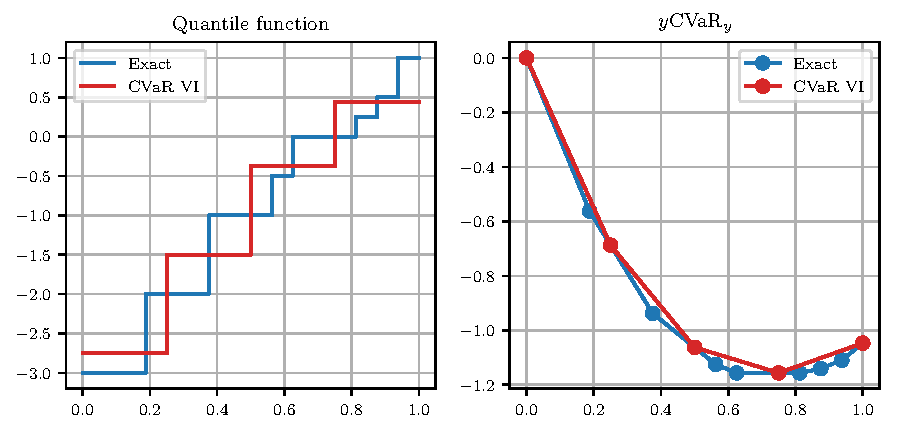
\includegraphics[width=0.8\linewidth]{gfx/cvar_visualized.pdf}
\caption{Comparison of a discrete distribution and it's approximation according to the CVaR linear interpolation operator.}
\label{fig:cvarvisual}
\end{figure}

\subsection{CVaR Computation via Quantile Representation}

We propose the following procedure: instead of using linear programming for the CVaR computation, we use the underlying distributions represented by the $y\cvar_y$ function to compute CVaR at each atom. The general steps of the computation are as follows

\begin{enumerate}
\item transform $y \cvar_y(Z(x'))$ of each reachable state $x'$ to a discrete probability distribution using \eqnref{varcvarderivation}.
\item combine these to to a distribution representing the full state-action distribution
\item compute $y \cvar_y$ for all atoms using \eqnref{varcvarintegration}
\end{enumerate}
See \figref{cvarcomputation} for a visualization of the procedure. 
\\
Note that this procedure is linear for discrete distributions. The only nonlinear step in the procedure is the sorting step in mixing distributions. Since the values are pre-sorted for each state $x'$, this is equivalent to a single step of the Merge sort algorithm, which means it is also linear in the number of atoms.

We show the explicit computation of the procedure for linearly interpolated atoms in \algref{cvarvi}.


\begin{figure}
\center
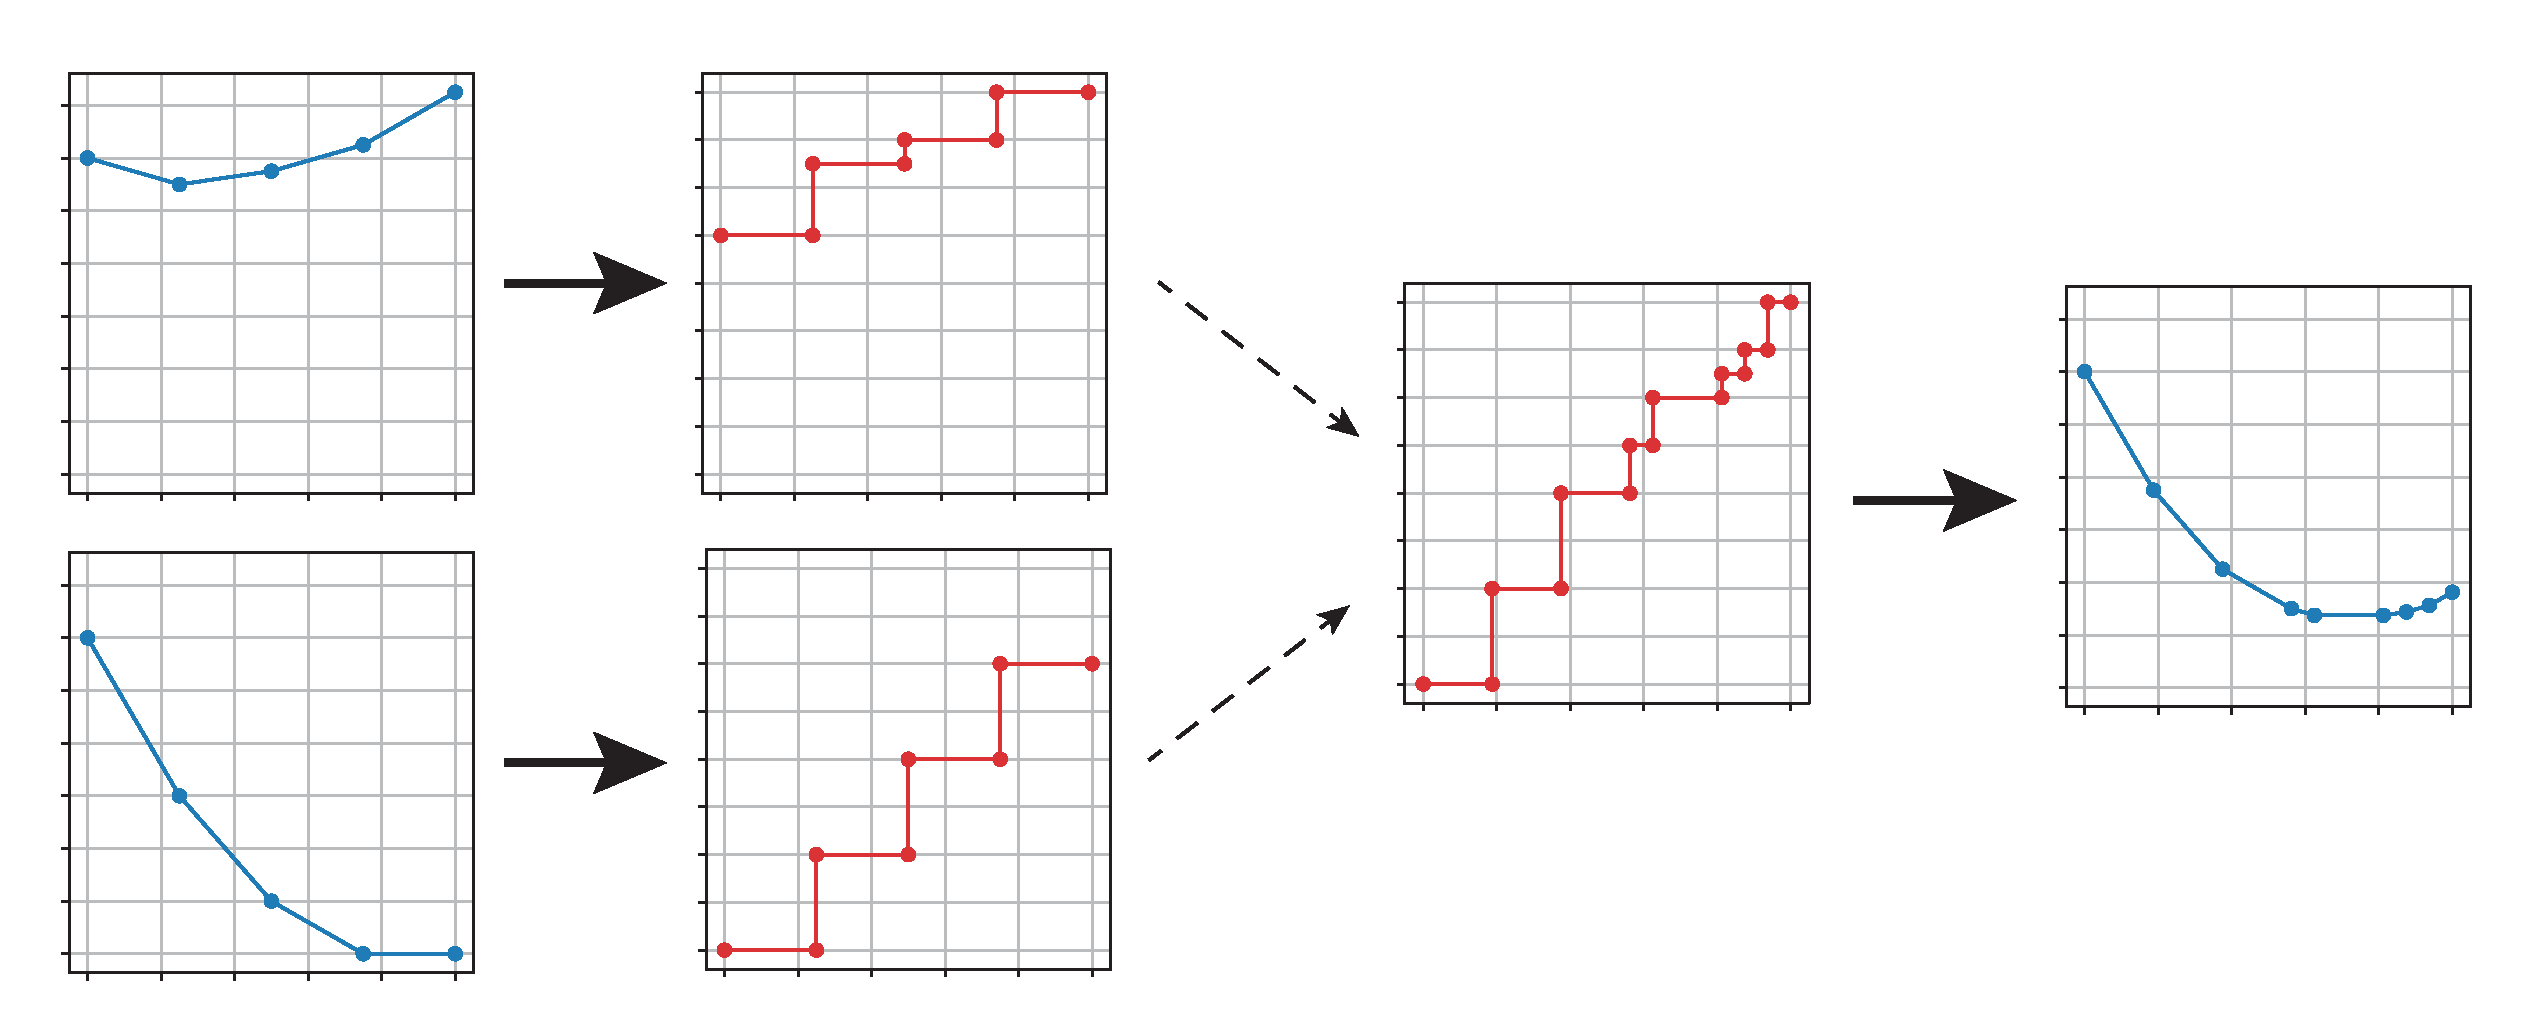
\includegraphics[width=\linewidth]{gfx/cvar_vi_conversion.pdf}
\caption{Visualization of the CVaR computation for a single state and action with two transition states. Thick arrows represent the conversion between $\ycvary$ and the quantile function.}
\label{fig:cvarcomputation}
\end{figure}

The proposed method draws remarkable similarity to distributional RL (\secref{prelim:distrl}). In fact, if we overlook the action selection phase, the one-step update is identical. The main differences between the two approaches are 1) action selection - in the distributional approach, we select a single action (based on the expected value) for the whole distribution contrary to CVaR Value Iteration, where we select a different action for each $\alpha$-level; 2) the approximation step - in distributional RL, we try to minimize the Wasserstein distance of selected distributions. In CVaR Value Iteration, we construct a distribution whose CVaRs at given confidence levels are identical to the exact distribution.

To show the correctness of this approach, we formulate it as a solution to problem \eqnref{cvardecomp} in the next section. Note that we skip the reward and gamma scaling for readability's sake. Extension to the Bellman operator is trivial.

\subsection{$\xi$-computation}

Similarly to \thmref{optimalpolicy}, we need a way to compute the $y_{t+1}=y_{t}\xi^*(x_t)$ to extract the optimal policy. We compute $\xi^*(x_t)$ by using the following intuition: $y_{t+1}$ is the portion of $Z(x_{t+1})$ that is present in $\cvar_{y_t}(Z(x_t))$. In the continuous case, it is the probability in $Z(x_{t+1})$ before the $\var_{y_t}(Z(x_t))$ as we show bellow.
\begin{theorem}
Let $x_1', x_2'$ be only two states reachable from state $x$ via action $a$ in a single transition. Let the cumulative distribution functions of the state's underlying distributions $Z(x_1'), Z(x_2')$ be strictly increasing with unbounded support.
Then the solution to minimization problem \eqnref{cvardecomp} can be computed by setting
\begin{equation}\label{eqn:xi-claim}
\xi ( x_i' ) = \dfrac{F_{Z(x_i')}\left(F^{-1}_{Z(x, a)}(\alpha)\right)}{\alpha} 
\end{equation}
\end{theorem}

\begin{proof}
Since we are interested in the minimal argument, we can ease the computation by focusing on the $\acvara$ function instead of $\cvar_\alpha$.
When working with two states, the equation of interest simplifies to
\begin{equation*}\label{eqn:cvardecomp2}
\begin{split}
\acvara(Z(x, a))&=\min_{\xi} \, p_1\xi_1\alpha \cvar_{\xi_1\alpha}\left(Z(x_1')\right) + p_2\xi_2\alpha\cvar_{\xi_2\alpha}\left(Z(x_2')\right)\\
\text{s.t.}& \quad p_1\xi_1 + p_2\xi_2 = 1\\
& 0 \le \xi_1 \le \frac{1}{\alpha}\\
& 0 \le \xi_2 \le \frac{1}{\alpha}
\end{split}
\end{equation*}
therefore
\begin{equation*}\label{eqn:cvardecomp3}
\begin{split}
\acvara(Z(x, a))&=\min_{\xi} \, p_1\xi_1\alpha \cvar_{\xi_1\alpha}(Z(x_1')) + (1-p_1)\dfrac{1-p_1\xi_1}{1-p_1}\alpha\cvar_{\frac{1-p_1\xi_1}{1-p_1}\alpha}(Z(x_2'))\\
&=\min_{\xi} \, p_1\int_0^{\xi_1\alpha}\var_{\beta}(Z(x_1'))\,\text{d}\beta + (1-p_1)\int_0^{\frac{1-p_1\xi_1}{1-p_1}\alpha}\var_{\beta}(Z(x_2')\,\text{d}\beta\\
\end{split}
\end{equation*}
To find the minimal argument, we find the first derivative w.r.t. $\xi_1$
\begin{equation*}
\begin{split}
\dfrac{\partial \acvara}{\partial \xi_1} &= p_1\alpha \var_{\xi_1\alpha}(Z(x_1')) + (1-p_1)\alpha\dfrac{-p_1}{1-p_1}\var_{\frac{1-p_1\xi_1}{1-p_1}\alpha}(Z(x_2')\\
&= p_1\var_{\xi\alpha}(Z(x_1')) - p_1\var_{\frac{1-p\xi}{1-p}\alpha}(Z(x_2'))
\end{split}
\end{equation*}
By setting the derivative to 0 , we get
\begin{equation*}
\var_{\xi_1\alpha}(Z(x_1')) \overset{!}{=} \var_{\frac{1-p\xi}{1-p}\alpha}(Z(x_2')) = \var_{\xi_2\alpha}(Z(x_2'))
\end{equation*}
\citet{bernard2015quantile} have shown that in the case of strictly increasing c.d.f. with unbounded support, it holds that
\begin{equation*}
\begin{split}
\var_{\xi_1\alpha}(Z(x_1')) &= \var_{\xi_2\alpha}(Z(x_2')) &&= \var_\alpha(Z(x, a))\\
F^{-1}_{Z(x_1')}(\xi_1\alpha) &= F^{-1}_{Z(x_2')}(\xi_2\alpha) &&= F^{-1}_{Z(x, a)}(\alpha)
\end{split}
\end{equation*}
and we can extract the values of $\xi_1\alpha, \xi_2\alpha$ using the 
\begin{equation*}
\begin{split}
&F^{-1}_{Z(x_1')}(\xi_1\alpha) &&= F^{-1}_{Z(x, a)}(\alpha) &&&/ \, F_{Z(x_1')}\\
&F_{Z(x_1')}\bround{F^{-1}_{Z(x_1')}(\xi_1\alpha)} &&= F_{Z(x_1')}\bround{F^{-1}_{Z(x, a)}(\alpha)}\\
&\xi_1\alpha &&= F_{Z(x_1')}\bround{F^{-1}_{Z(x, a)}(\alpha)}
\end{split}
\end{equation*}
And similarly for $\xi_2$.

Since the problem is convex, we have found the optimal point.

\end{proof}

The theorem is straightforwardly extendable to multiple states by induction. We conjecture that similar claim holds for general distributions, however this would require more technical arguments and is out of scope of this thesis. Among other difficulties, the optimal $\xi$ is not unique for general distributions. See \citet{bernard2015quantile} for details on the two-dimensional case for general distributions.

%*****************************************



\section{Experiments}\label{sec:vi:experiments}

We test the proposed algorithm on the same task as \citet{chow2015risk}. The task of the agent is to navigate on a rectangular grid to a given destination, moving in it's four-neighborhood. To encourage fast movement towards the goal, the agent is penalized for each step by receiving a reward -1. A set of obstacles is placed randomly on the grid and stepping on an obstacle ends the episode while the agent receives a reward of -40.
To simulate sensing and control noise, the agent has a $\delta=0.05$ probability of moving to a different state than intended.

For our experiments, we choose a $40 \times 60$ grid-world and approximate the $\acvara$ function using 21 log-spaced atoms with $\theta=2$ as in \citep{chow2015risk}. The learned policies on a sample grid are shown in \figref{vigrid}.

While \citet{chow2015risk} report computation time on the order of two hours, our naive Python implementation converged within 20 minutes and there is ample room for improvement.

\begin{figure}[h]
\center
\makebox[\textwidth][c]{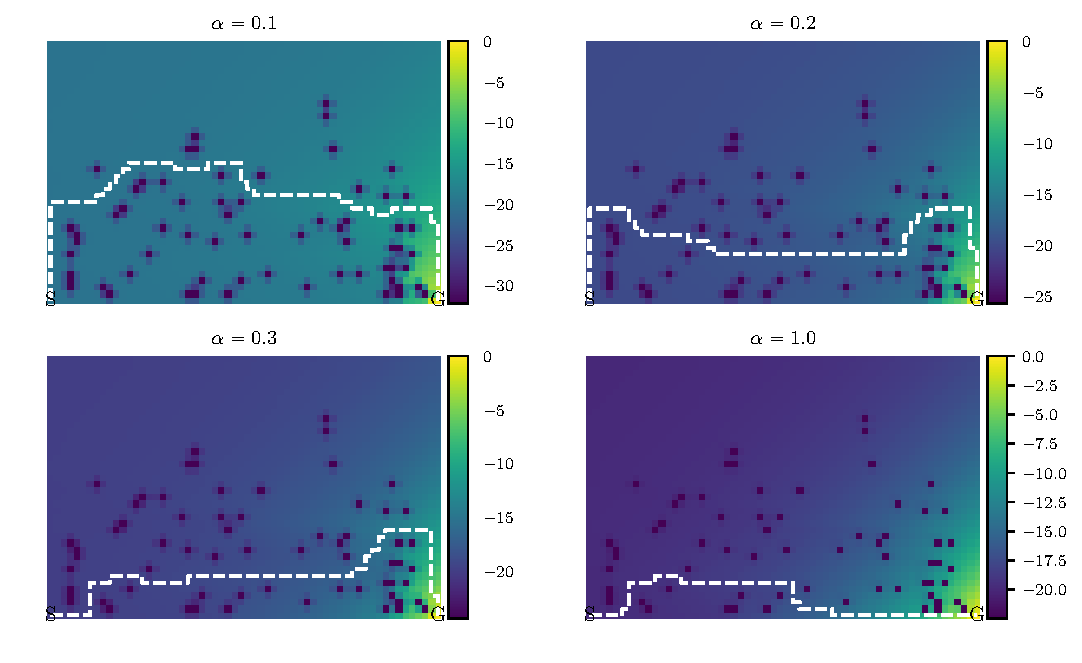
\includegraphics[width=1.1\linewidth]{gfx/vi_optimal_paths.pdf}}
\caption{Grid-world simulations. The optimal deterministic paths are shown together with CVaR estimates for given $\alpha$. \todo{another plot here}}
\label{fig:vigrid}
\end{figure}

\subsection{Empirical difficulties}
We have encountered slight difficulties when testing the algorithms. While the CVaR value estimates monotonically converged towards the contraction fixed points, the same cannot be said about the extracted policies. Some policies failed to reach the goal via the optimal paths and some even got stuck in cycles.

After some investigation, we identified that these nonoptimal behaviors happen around points where a small $\alpha-$change affects the selected actions and are caused by the approximation errors around those points. We note that similar problems also affect the distributional RL approaches, as one can find examples of distributions whose expected value differs dramatically from the value approximated by the Wasserstein optimum.

These problems can always resolved by increasing the number of atoms around these critical points, as both methods are consistent in the limit.


\begin{algorithm}
\caption{CVaR Computation via Quantile Representation}
\begin{algorithmic}\label{alg:cvarvi}
\setlength{\columnseprule}{0.4pt}
\begin{multicols}{2}
\STATE \textbf{function} extractDistribution
\bindent
    \STATE \textbf{input:} vectors $\mathbf{C}, \mathbf{y}$
    \STATE \comment{Note: $y_0 = C(x', y_0) = 0$}
    \FOR{$i \in \braces{1, ..., |\mathbf{y}|}$}
	\STATE $d_i = \dfrac{C(x', y_i)-C(x', y_{i-1})}{y_i-y_{i-1}}$
	\ENDFOR
	\STATE \textbf{output} vector $\mathbf{d}$
\eindent
\STATE \textbf{function} extractC
\bindent
    \STATE \textbf{input:} vectors $\mathbf{d}, \mathbf{p}$
    \STATE $C_0 = 0$
    \FOR{$i \in \braces{1, ..., |\mathbf{p}|}$}
	\STATE $C_i = C_{i-1} + d_i \cdot p_i$
	\ENDFOR
	\STATE \textbf{output} vector $\mathbf{C}$
\eindent
\end{multicols}

\hrulefill

\STATE \textbf{function} mixDistributions
\bindent
    \STATE \textbf{input:} tuples $(\mathbf{d^{(1)}}, p^{(1)}),...,(\mathbf{d^{(K)}}, p^{(K)})$ and vector $\mathbf{y}$ 
    \STATE \comment{$\sum_{k=1}^{K}p_k = 1$}
    \FOR{$i, k \in \braces{1, ..., K} \times \braces{1, ..., |\mathbf{y}|}$}
    	\STATE \comment{Weigh atom probabilities by transitions}
		\STATE $p^{(k)}_i = p^{(k)} \cdot (y_i - y_{i-1})$
	\ENDFOR
	\STATE \comment{Join all tuples together:}
	\STATE $atoms = \braces{(d^{(1)}_1, p^{(1)}_1), ..., (d^{(1)}_N, p^{(1)}_N), (d^{(2)}_1, p^{(2)}_1), ..., (d^{(K)}_N, p^{(K)}_N)}$
	\STATE Sort $atoms$ by $d$
	\STATE Unwrap vectors $\mathbf{d}, \mathbf{p}$ from sorted tuples
	\STATE \textbf{output} $\mathbf{d}, \mathbf{p}$
\eindent
\\\hrulefill
\STATE \comment{Main}
\STATE \textbf{input:} tuples $(C(x_i', \bigcdot), p^{(1)}),...,(C(x_i', \bigcdot), p^{(K)})$ and vector $\mathbf{y}$ 
\FOR{$i \in \braces{1, ..., K}$}
\STATE $\mathbf{d^{(i)}}$ = extractDistribution($C(x_i', \bigcdot), \mathbf{y}$)
\ENDFOR
\STATE $\mathbf{d_{mix}}, \mathbf{y_{mix}} =$ mixDistributions($(\mathbf{d^{(1)}}, p^{(1)}),...,(\mathbf{d^{(K)}}, p^{(K)}), \mathbf{y}$)
\STATE $\mathbf{C_{out}} =$ extractC($\mathbf{d_{mix}}, \mathbf{y_{mix}}$)
\STATE \textbf{output:} $\mathbf{C_{out}}$
\end{algorithmic}

\end{algorithm}


%\section{Summary}
%
%In this chapter, we have extended the CVaR Value Iteration algorithm and improved it's computation complexity from polynomial (each step required computing a Linear Program) to linear in the number of discretized atoms.




%*****************************************
%*****************************************
%*****************************************
%*****************************************
%*****************************************



